% coding:utf-8

%FOSAET, a LaTeX-Code for a electrical summary of basic electronics
%Copyright (C) 2013, Daniel Winz, Ervin Mazlagic, Mario Felder

%This program is free software; you can redistribute it and/or
%modify it under the terms of the GNU General Public License
%as published by the Free Software Foundation; either version 2
%of the License, or (at your option) any later version.

%This program is distributed in the hope that it will be useful,
%but WITHOUT ANY WARRANTY; without even the implied warranty of
%MERCHANTABILITY or FITNESS FOR A PARTICULAR PURPOSE.  See the
%GNU General Public License for more details.
%----------------------------------------

\subsection{Drain Schaltung}
\begin{figure}[h!]
	\centering
	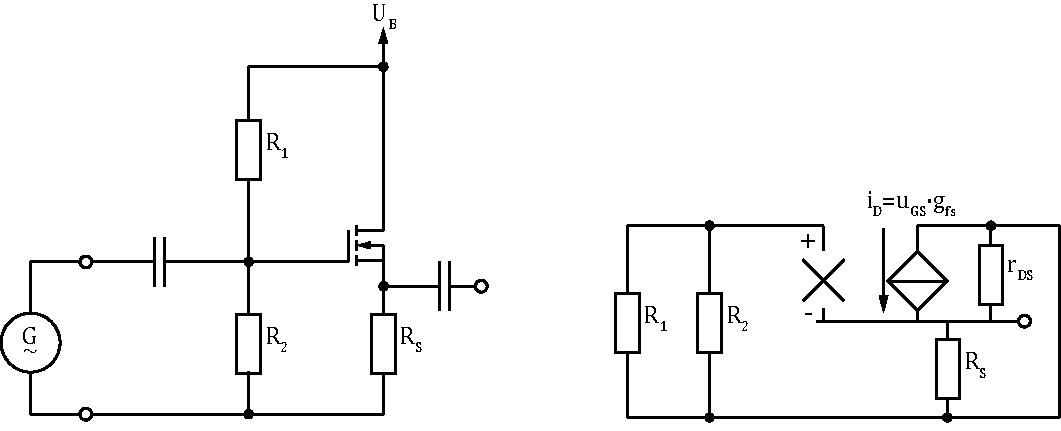
\includegraphics[width = \linewidth]{../fig/fet_drain.pdf}
	\caption{Drain Schaltung und Kleinsignalersatzschaltung}
	\label{fet:drainschaltung}
\end{figure}
\noindent
Spannungsverstärkung:
\[
	V_u = \frac{r_{DS} \parallel R_S}{r_{DS} \parallel R_S + \frac{1}{g_{fs}}} \approx 1
\]
Ausgangswiderstand:
\[
	r_a = \frac{1}{g_{fs}} \parallel r_{DS} \parallel R_S
\]
Eingangswiderstand:
\[
	r_e = (r_{GS} \cdot R_S \cdot g_{fs} + R_S + r_{GS}) \parallel R_1 \parallel R_2
\]
für $r_{GS} = \infty$:
\[
	r_e = R_1 \parallel R_2
\]
